\documentclass[12 pt,twopage]{article}
\usepackage{amsmath,amssymb,amsfonts,amsthm}
\usepackage[english]{babel}
\usepackage[utf8]{inputenc}
\usepackage{fancyhdr}
%\usepackage[a3paper]{geometry}
\usepackage{geometry}
\usepackage{tikz}
\usepackage{xcolor}
\usepackage{float}
\usepackage{bm}
\usepackage{listings}
\usepackage{xcolor}
\usepackage{algorithm2e}
\usepackage{tikz}
\usetikzlibrary{automata,positioning}

\lstset{basicstyle=\ttfamily,
 showstringspaces=false,
 commentstyle=\color{gray},
 keywordstyle=\color{blue},
 morekeywords={grep, head, tail, cut }
}

\newcommand{\codepath}{../}
\newcommand{\scriptpath}{../scripts}

\newcommand{\hr}{\begin{center} \line(1,0){450} \end{center}}
\newcommand{\R}{\mathbb R}
\newcommand{\B}{ \{0,1\} }
\newcommand{\tr}{^\mathsf{T}}
\newcommand{\F}{\mathcal{F}}
\newcommand{\norm}[1]{\left\lVert#1\right\rVert}
\DeclareMathOperator{\Id}{Id}
\DeclareMathOperator{\diag}{diag}
\DeclareMathOperator{\epi}{epi}
\DeclareMathOperator{\co}{co}
\DeclareMathOperator{\interior}{int}
\DeclareMathOperator{\Proj}{Pr}
\DeclareMathOperator*{\argmin}{argmin}
\DeclareMathOperator*{\argmax}{argmax}
\newcommand{\midd}{\mathrel{}\middle|\mathrel{}}


\newcommand{\generalPdfSymbol}{\bm{p}}
\newcommand{\gps}{\generalPdfSymbol}
\newcommand{\bernoulliPdfSymbol}{p_{bern}}
\newcommand{\binomialPdfSymbol}{p_{bin}}

\newcommand{\s}[1]{\sum_{#1}}
\newcommand{\am}[2]{\argmax\limits_{#1} #2}
\newcommand{\partition}[2]{\{ #1_1, #1_2, \dots, #1_{#2} \} }
\newcommand{\pd}[2]{#1 \left( #2 \right) }
\newcommand{\p}[1]{\pd{P}{#1}}
\newcommand{\cp}[3]{\pd{#1}{#2 \midd #3}}
\newcommand{\cpf}[3]{ \frac{\pd{#1}{#2,#3}} { \pd{#1}{#3} } }
\newcommand{\cpeq}[3]{\cp{#1}{#2}{#3} = \cpf{#1}{#2}{#3}}

\newcommand{\ltp}[3]{\s{#2_j \in \partition{#2}{n} } \cp{#1}{#3}{#2_j} \p{#2_j} }
\newcommand{\bysNom}[3]{\cp{#1}{#3}{#2_i} \pd{#1}{#2_i} }
\newcommand{\bys}[3]{ \frac{\bysNom{#1}{#2}{#3} }{ \ltp{#1}{#2}{#3} } }
\newcommand{\byseq}[3]{}


\newcommand{\bernoulli}[2]{ #1^{#2} \left(1 - #1\right)^{1 - #2}  }
\newcommand{\bern}{\bernoulli{\phi}{c}}

\newcommand{\likelihood}[1]{\prod\limits_{c \in C} #1 }


%\geometry{top=20mm, left=20mm, right=10mm, bottom=15mm}

\pagestyle{fancy}
\lhead{Christian Lengert 153767}
\rhead{\today}
\chead{Graphical Models Lab}
\rfoot{Page \thepage}

 \setlength{\parindent}{0pt}
\begin{document}

\begin{abstract}

 In this article we will explore the model of Latent Dirichlet Allocation theoretically by introducing the model and multiple algorithms for model selection and inference and practically by implementing an inference algorithm based on Gibb's sampling and exploring and visualizing the results.
 The first section will give an overview about the model and the domain of problems it is applied to.
 The second section explains how to implement the model-selection algorithm and will guide the way to  .
 In the third section we will train the model on a subset of the simple english wikipedia and evaluate the results by visualizing the learned topics with the Python library pyLDAviz.
\end{abstract}

%\twocolumn
\section{Latent Dirichlet Allocation}
The model of Latent Dirichlet Allocation (LDA) is a generative probabilistic model for collections of discrete data proposed by Blei, Ng and Jordan \cite{Blei2003}. It is a mixture model that tries to model latent topics or concepts of multinomial observations, e.g. words in text corpus.

\begin{figure}[h]
 \begin{center}
  \begin{footnotesize}
   \begin{description}
    \item[\( K \)] : Number of topics to be found by the model
    \item[\( M \)] : Number of documents in the corpus
    \item[\( V \)] : Number of unique terms in the dictionary
    \item[\( \vec\alpha \in \mathbb{R}^K \)] : Hyperparameter of the document-topic Dirichlet distribution
    \item[\( \vec\beta \in \mathbb{R}^V \)] : Hyperparameter of the topic-word Dirichlet distribution
    \item[\( \vec\vartheta_m \in \mathbb{R}^K \)] : Topic distribution of each document \(m\).
    \item[\( \vec\phi_k \in \mathbb{R}^V \)] : Term distribution of each topic \(k\).
    \item[\( N_m \)] : The length of the m-th document.
    \item[\( z_{m,n} \)] : Topic index for the \(n\)-th word in document \(m\).
    \item[\( w_{m,n} \)] : the \(n\)-th word in document \(m\).
   \end{description}
  \end{footnotesize}
 \end{center}
 \caption{Notation}
 \label{fig:notation}
\end{figure}

To understand the structure of the model we will look at the Likelihood-function for
The probability of a term to occur in a document \(p \left( w=t \right)\) is modeled as a marginal distribution of the joint distribution over topics and terms.
\onecolumn
%\begin{equation}
% p\left( w=t \right) = \sum\limits_{k} p\left( w=t \midd z=k \right) p\left( z=k \right)
%\end{equation}

\begin{equation*}
 p\left( \vec{w}_{m}, \vec{z}_{m}, \vec{\vartheta}_{m} \midd \vec{\alpha}, \vec{\beta} \right) = \prod\limits_{w_{m,n}}^{N_m} p \left(w_{m,n} \midd \vec\phi_{z_{m,n}} \right) p \left(z_{m,n} \midd \vec\vartheta_{m} \right) p\left( \vec\vartheta_m \midd \vec\alpha \right) p \left( \phi \midd \vec\beta \right)
\end{equation*}

%bag of words
%documents plate
%corpus plate
\subsection{Generative Process}
To understand the model better we analyze the LDA generative model. To generate a corpus consisting of documents, that consist of words, the steps shown in figure \ref{fig:generativeProcess} have to be taken.

Given the number of topics \(K\), the number of documents \(M\), the Dirichlet-hyperparameters \(\alpha,\beta\) and the moment of the Poisson distribution \( \xi \) we start by specifiying the topics by sampling a categorical topic-word distribution for every topic. These hold a probability for every possible term to occur in the context of the topic. We sample the topic-categoricals from a Dirichlet distribution with the parameter \(\beta\).

With the Dirichlet-samples we can start to generate documents. For every document \( d \) we sample from a Dirichlet distribution again, this time using with the hyperparameter \( \alpha \). The resulting categorical distribution sets probabilities for all topics to be included in the documents. Furthermore we sample a document length from the Poisson distribution.

Finally, for every word to be generated, we sample a topic index from the documents own document-topic-categorical distribution and then sample the term given the

Look in section \ref{code:generativeModel} for an implementation of the process.
\onecolumn
\begin{figure}[h]
 \begin{center}
  \begin{algorithm}[H]
   \KwData{Number of topics \(K\), Number of Documents \(M\), Dirichlet parameters \(\alpha\) and \(\beta \), Poisson parameter \(\xi\)}
   \KwResult{Corpus \( c \)}
   \For{all topics \(k \in [1,K] \) }{
    sample topic-term distribution parameters \( \phi_k \sim Dir \left( \beta \right) \)
   }
   \For{ all documents \( m \in [1,M] \)}{
    sample document-topic distribution parameters \( \vartheta \sim Dir \left( \alpha \right) \)\\
    sample document-length \(l_m \sim Poisson \left( \xi \right) \)\\
    \For{ all words \( w \in [1,l_m] \)}{
     sample topic index \( z_{m,n} \sim Mult\left( \xi \right)\)\\
     sample term for word \( w_{m,n} \) from \( p\left( w_{m,n} \midd z_{m,n}, \beta \right)\) \( w_{m,n} \sim Mult\left( \phi_{z_{m,n}} \right) \)
    }
   }
   
  \end{algorithm}
  \caption{The generative model of LDA  \cite{Blei2003,Heinrich2005}}\label{fig:generativeProcess}
 \end{center}
\end{figure}
\subsection{Model Selection}

\subsubsection{algorithm}
Various algorithms to tackle the inference problem for LDA have been proposed \cite{Blei2003}. In this report we will focus on a specific Markov-Chain Monte-Carlo based method, namely a Gibb's sampler. We will execute the inference with the algorithm explained by Pefta et. al.
%describe algorithm
%what are hyperparameteres
%what are cojugate priors
\section{Imlementation}
Although the inference algorithm can potentially be parallelized in multiple ways \cite{Newman2006ScalablePT,Wang2009PLDAPL}, we aim to create a serial implementation for to strive for correctness instead of performance.
\subsection{Preparation}
First we have to choose a text corpus to estimate the parameters of the LDA-model from. For this we use a dump from the simple english wikipedia \cite{simplewi84:online}, namely the version named 'All pages, current versions only'.

For the purpose of speeding up the development process we will perform our operations on an even smaller subset of only 5 articles, to avoid long loading times on every run. We split some articles of the downloaded file into a smaller file with the script in section \ref{extract}.

\subsection{Class : Dataset}
We aggregate all operations regarding the preprocessing of the corpus in a class named Dataset, which can be examined in section  \ref{class:dataset}. Our goal here is to process all articles and end up with a datatructure that provides us with with counts of terms for every document. Therefore we have to establish a common dictionary containing all occurring words from all documents and process

\subsection{Class : LDA}

\section{Evaluation}
To evaluate the topics that the model has learned in the trainingprocess on the wikipedia dataset we will use the Python package PyLDAviz. The plots of the first six found topics can be found in the figures \ref{fig:t12}, \ref{fig:t34} and \ref{fig:t56}. All plots show an intertopic distance map on the left side and a histogram on the right side. The distance map is a two dimensional projection of the topic space computed with a multidimensional scaling algorithm \cite{Sievert2014}. The Histogram shows the most frequent terms for the chosen topic in descending order, in which the the red bar shows the term frequency in the topic and the blue bar the overall term frequency.
The model in use is trained for 50 iterations on the first 10000 artices of the dataset consiting of \( 196934 \) documents.
\bigbreak
To try to find a possible semantic we will take a look at the most frequent terms in the topics.

\paragraph{Topic 1}
The first topic contains many terms related to the internet, communcation and publication. The five most frequent terms are \enquote{title},\enquote{http},\enquote{cite},\enquote{url} and \enquote{web}.
\paragraph{Topic 2}
\paragraph{Topic 3}
\paragraph{Topic 4}
\paragraph{Topic 5}
\paragraph{Topic 5}


\begin{figure}
 \begin{subfigure}[c]{1\textwidth}
  \caption{Topic 1}
  \centering
  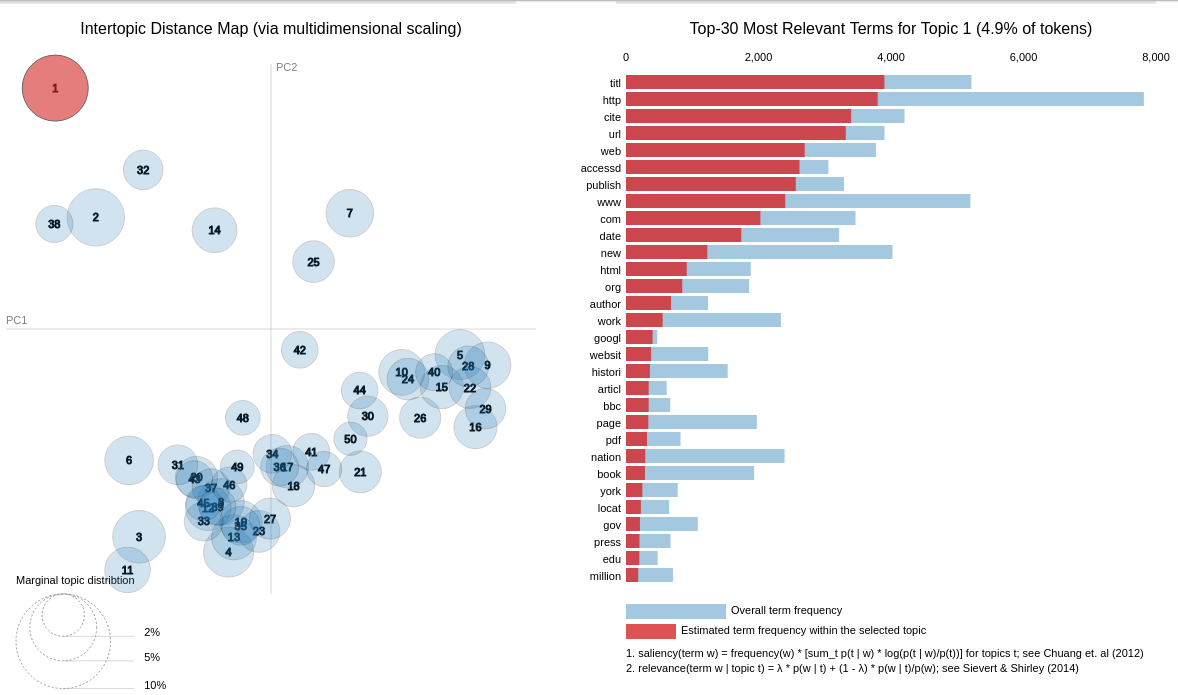
\includegraphics[width=.9\linewidth]{\gpath/t1.png}
 \end{subfigure}
 \begin{subfigure}[c]{1\textwidth}
  \caption{Topic 2}
  \centering
  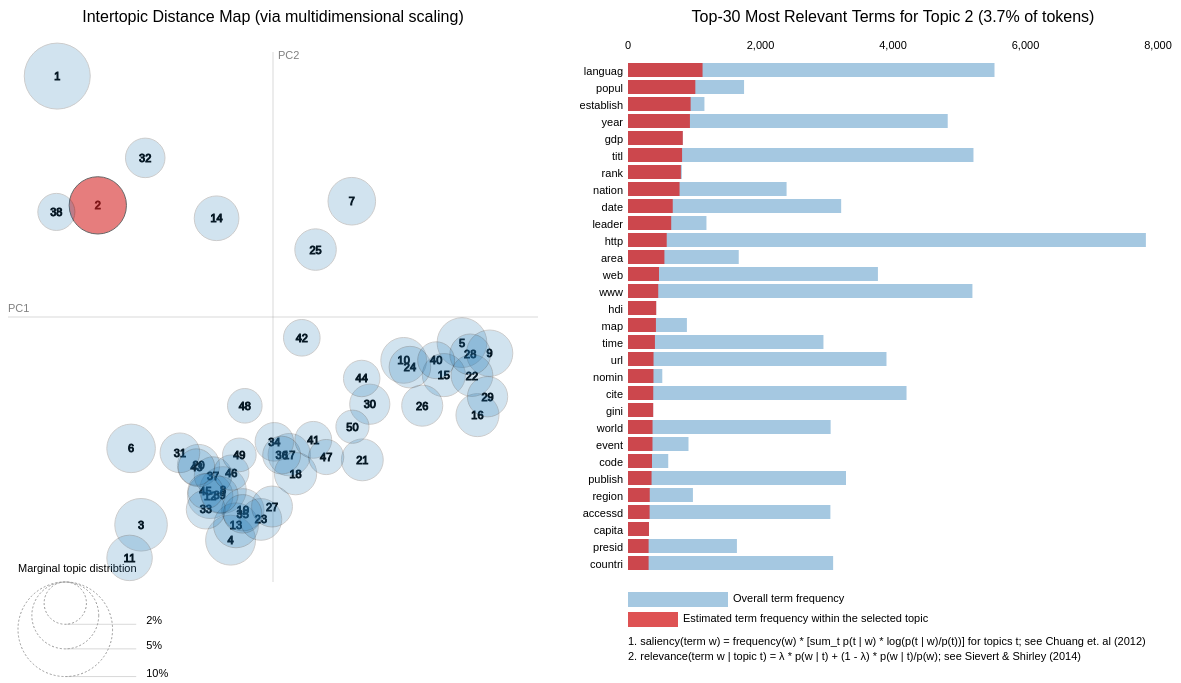
\includegraphics[width=.9\linewidth]{\gpath/t2.png}
 \end{subfigure}
 \caption{Plots of the first six topics}
 \label{fig:t12}
\end{figure}


\begin{figure}
 \begin{subfigure}[c]{1\textwidth}
  \caption{Topic 3}
  \centering
  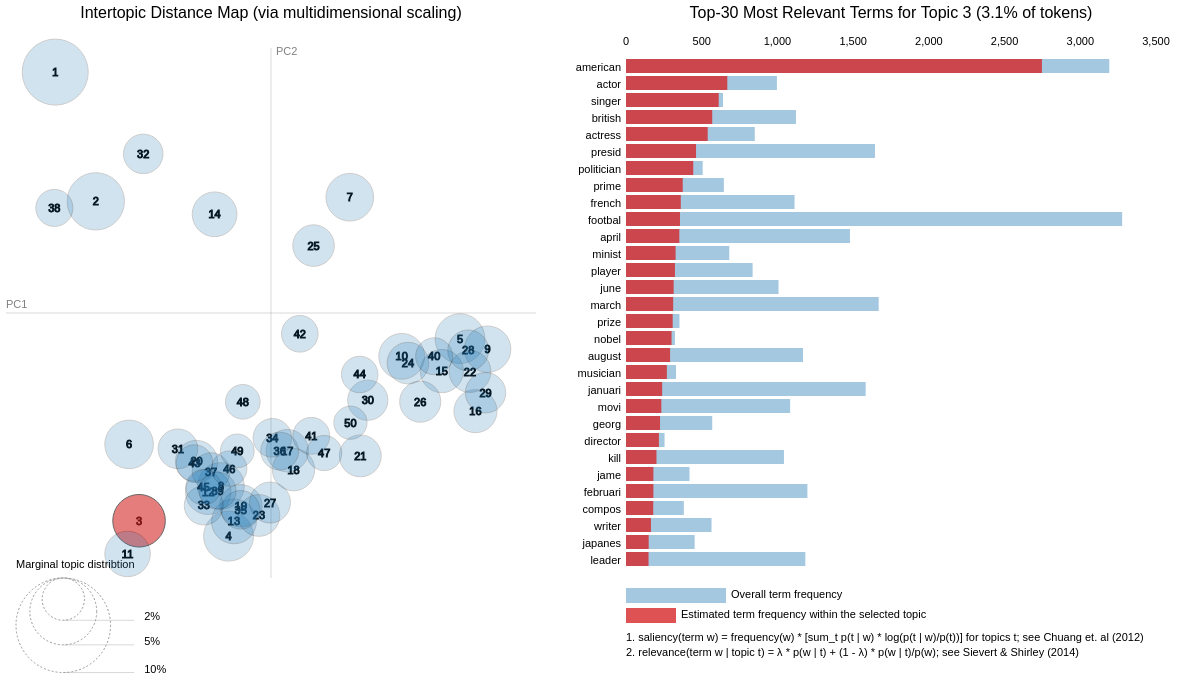
\includegraphics[width=.9\linewidth]{\gpath/t3.png}
 \end{subfigure}
 \begin{subfigure}[c]{1\textwidth}
  \caption{Topic 4}
  \centering
  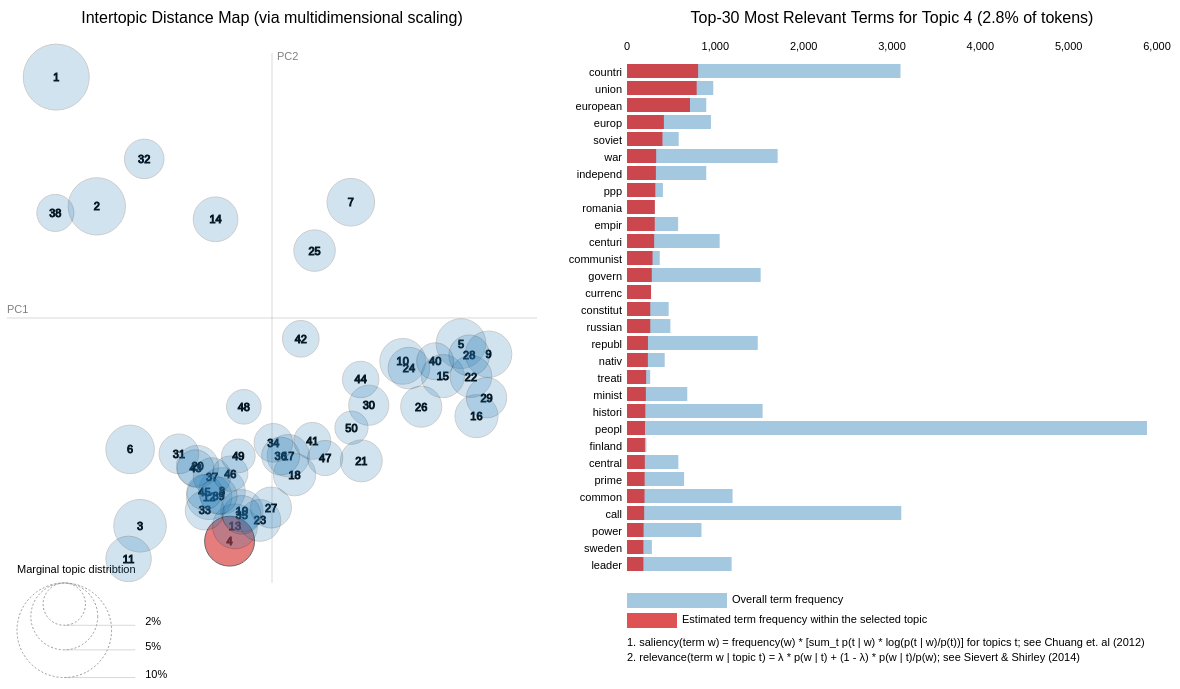
\includegraphics[width=.9\linewidth]{\gpath/t4.png}
 \end{subfigure}
 \caption{Plots of topic 3 and 4}
 \label{fig:t34}
\end{figure}


\begin{figure}
 \begin{subfigure}[c]{1\textwidth}
  \caption{Topic 5}
  \centering
  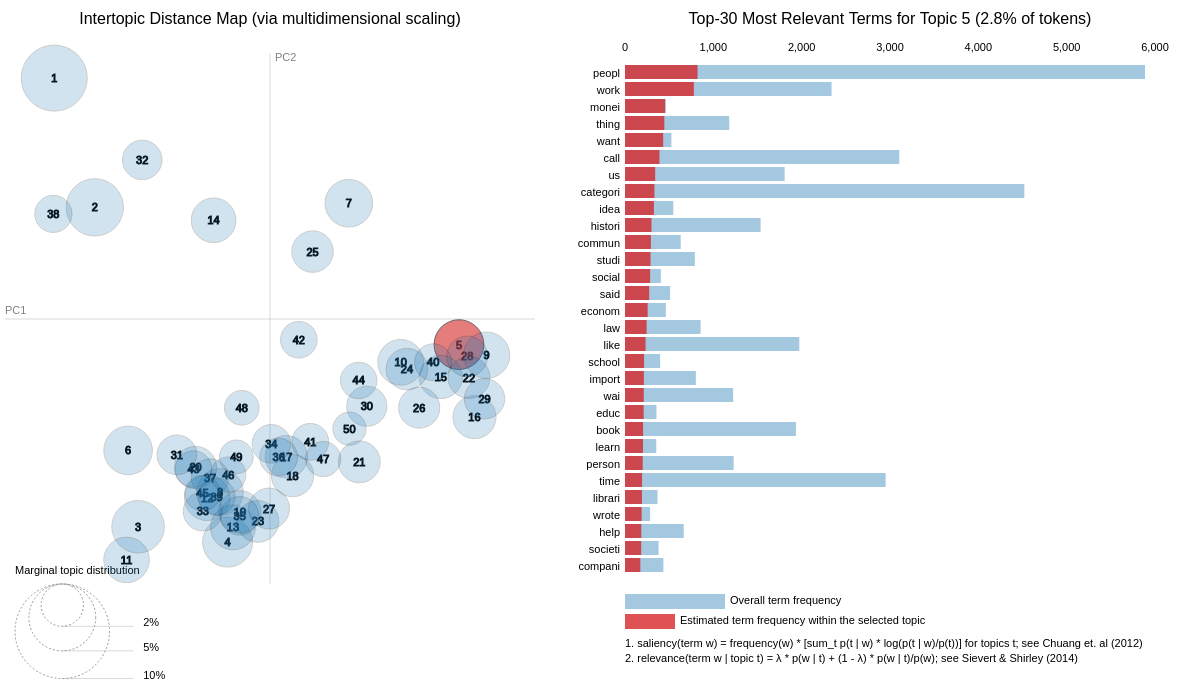
\includegraphics[width=.9\linewidth]{\gpath/t5.png}
 \end{subfigure}
 \begin{subfigure}[c]{1\textwidth}
  \caption{Topic 6}
  \centering
  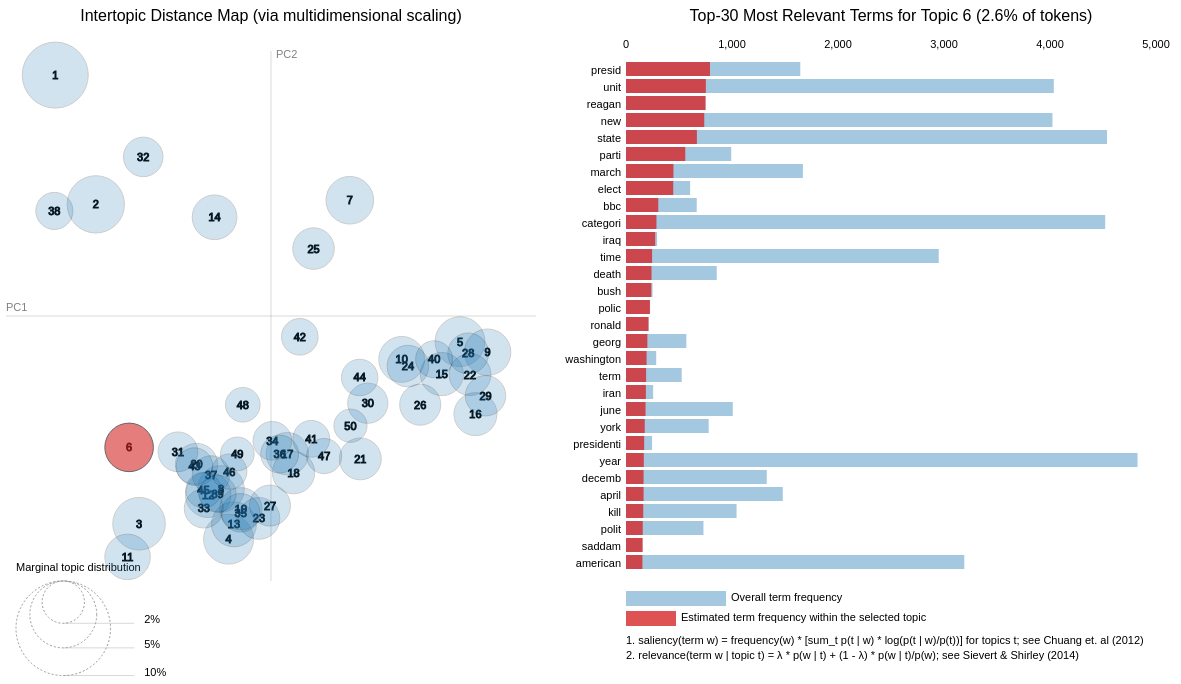
\includegraphics[width=.9\linewidth]{\gpath/t6.png}
 \end{subfigure}
 \caption{Plots of the first six topics}
 \label{fig:t56}
\end{figure}






\newpage

\bibliography{refs}
\bibliographystyle{IEEEtran}

\newpage
%\onecolumn
\section{Appendix}
\subsection{Extract subset} \label{extract}
\lstinputlisting[language=bash]{\scriptpath/extractSmallSubset.bash}

\subsection{Class : Dataset} \label{class:dataset}
\lstinputlisting[language=python]{\codepath/lda/dataset.py}

\subsection{Class : LDA} \label{class:lda}
\lstinputlisting[language=python]{\codepath/lda/inference.py}

\subsection{Class : LDA} \label{code:generativeModel}
\lstinputlisting[language=python]{\codepath/lda/generativeModel.py}


\end{document}
